
\section{Experimental Methodology}\label{sec:methods}

\subsection{Testbed and Scenarios}\label{sec:testbed}

The security and correctness experiments use a deterministic discrete-event testbed with four cells of one gateway and six devices (one legacy device per gateway), 1~Hz per device for 300~s (7200 observations per run) and a 180~s drain. Gateways implement durable store-and-forward (2~s retransmission timeout, 60 messages/s backlog drain, unbounded buffers with a backlog limit in messages, not bytes, acknowledgement once the verifier has ingested an entry), and the network adds 20~ms plus exponential jitter and injects faults per scenario (Table~\ref{tab:scen}). Protocol time is virtual; processing cost is measured in wall-clock time. Separate generators for production, network, attacker decisions and rendering, all derived from one seed, give every pipeline identical schedules (hence paired comparisons); attacks are rendered into each pipeline's wire format using only the keys the attacker holds. A sixteenth, \emph{mixed} workload combines all attack and failure classes with a 120~s horizon, a device move with a policy update and a revocation with a compromise window.

\begin{table}[!htbp]
\caption{Scenarios (\RScenarioSeeds\ paired seeds each in the main evaluation; virtual duration 300~s).\label{tab:scen}}
\begin{adjustwidth}{-\extralength}{0cm}
\footnotesize
\begin{tabularx}{\fulllength}{l>{\raggedright\arraybackslash}X}
\toprule
\textbf{Id} & \textbf{Injection}\\
\midrule
E1 & no faults\\
E2 / E3 & broker modifies 5\% of payloads / 2\% each of asset, timestamp and sequence or message identifier\\
E4 & 100 injections by an unknown producer; 100 forgeries for cell-3 devices relayed through compromised gateway 2\\
E5 & stolen keys of two devices injected at the broker (100); device key plus relay key: back- and front-running equivocation (10\% each), gap-fill (10\%), full impersonation from 150~s\\
E6 & exact replays (5\% of messages, 5--150~s later) and timestamp-refreshed replays (3\%)\\
E7 / E8 & redelivery 10\%, acknowledgement loss 10\%, loss 2\% / benign sequence-reuse firmware fault on two devices (two occurrences each)\\
E9 / E10 & 30\% of messages delayed up to 3~s / 2\% delayed 30--90~s plus clock freeze (5~s) and backward step (30~s) on four devices\\
E11/E12 / E11b & 120~s gateway partition with device reboot, gateway restart during the drain and 5\% acknowledgement loss / 150~s partition with a 120~s admission horizon\\
E13 & short-lived workload credentials (90~s validity, renewal every 60~s) and device key rotation during a 120~s partition\\
E14 & device and gateway keys of cell 4 compromised at 120~s (impersonation, legacy forgery); revocation at 200~s with $t_\mathrm{comp}=120$~s, re-keying at 205~s; attacks with the revoked keys continue\\
E15 & compromised gateway: forgeries for its own devices, suppression of 5\% of messages, replays\\
E16 & insider tampering classes T1--T7 applied after E5 runs, followed by an offline audit (\RAuditTamperSeeds\ seeds)\\
\bottomrule
\end{tabularx}
\end{adjustwidth}
\end{table}

\subsection{Pipelines and Review Schedules}\label{sec:pipelines}

All pipelines share storage, downstream processing and the policy document and differ in admission and conflict-response semantics (repository \texttt{docs/BASELINES.md}). \textbf{B1 (conventional)} authenticates the gateway TLS session once, permits plant-wide publication, de-duplicates message identifiers within 300~s and upserts by (device, timestamp). \textbf{B2 (Zero Trust)} verifies the workload credential, the path-bound policy of \sys\ and freshness per message, without object signatures. \textbf{B3 (provenance)} verifies origin signatures without rotation grace and keeps a hash-chained ledger, approximating signature and hash-chain provenance schemes~\cite{hasan2009tos,javaid2018blockpro,sigwart2019bcprov}. \textbf{B4 (mainstream combination)} adds to B2 origin signatures on the observation statement, rotation grace, first-writer-wins admission on the producer-assigned event identity, as CloudEvents keys on it~\cite{cloudevents102}, and B3's ledger, but no relay statement, predecessor-link contest, quarantine workflow or taint.

\textbf{B5 (feed-level comparator)} keeps every mechanism of \sys\ except the conflict response: a receipt that adds new fork evidence (a second admitted content for its identity, an admitted successor link naming another digest for it, or a predecessor link naming none of the admitted versions of its predecessor, as in SSB and PeerReview~\cite{tarr2019ssb,haeberlen2007peerreview}) holds the affected (device, epoch) feed from the fork point onward; every held observation is a review case, and an automated reviewer releases held and releasable quarantined observations that satisfy the hash-link corroboration rule of Section~\ref{sec:lifecycle}. All B5 and B5s results of the simulation stages come from the corrected implementation of this specification (Section~\ref{sec:impl}); the historical results are kept in Document S1 and Data S1. A released held observation does not re-run admission, which it had passed on arrival, and a feed resumes only when none of its hold cases is undecided; because every new arrival on a forked feed opens a case younger than $R$, under a slow schedule a forked feed does not resume before production ends (in E5 with \Bhist, seeds 21--23: forks at 30--50~s, resumption at 360--370~s, after production ended at 300~s), so B5's withholding reflects both the schedule and this resume rule. Within a periodic pass, cases are reviewed in identity order, which lets a released predecessor corroborate its successor in the same pass, for B5 and PBTI-R alike; contested identities get no case. Because B5 adds a hold condition to the authority predicate of \sys\ and releases a held observation only when Rule L commits it and a hash link corroborates it, its authoritative set is never larger than that of PBTI-R with the same reviewer and schedule: it can retain fewer, but never more, forgeries and withhold more, but never less, genuine data (no outcome violated it in any of the \XSubsetRuns\ matched runs), so the matched comparison measures the size of these differences, not their sign.

The reviewer is our design and its schedule a parameter of the comparison. The \emph{one-shot} rule rejects an uncorroborated case at its first review and runs with minimum case age $R=60$~s and review cadence $C=10$~s (\Bhist); the \emph{deferring} rule keeps an uncorroborated, uncontradicted case pending and runs with $R\in\{0,1,5,60\}$~s and $C\in\{1,10\}$~s; and \emph{event-driven} review (\Bev) re-examines, right after an admission, the cases whose evidence it can have changed ($R=0$ with a periodic scheduler is not event-driven). \textbf{B5s} disables recovery and keeps the feed hold (the SSB rule). \textbf{PBTI-R} applies the same reviewer and schedules to the quarantine cases of \sys\ (\Rhist, \Rev), so PBTI-R versus B5 under the same schedule is the matched-review comparison, whereas \sys\ versus B5 also differs in active recovery. \textbf{PBTI-SH} adds selective evidence-gated holds to \sys: from its first contested identity a feed is suspect for the rest of the epoch, and a committed observation of a suspect feed that no admitted successor link corroborates is withheld, retroactively, until such a link arrives or, in the variant PBTI-SH-T30, until a 30~s timeout; contested or tainted observations are never released, and no evidence source is added.

\subsection{Outcomes}\label{sec:metrics}

At the end of each run the oracle counts non-legitimate authoritative observations (O1: content matching no legitimate observation) and legitimate observations produced by honest devices and accepted by a gateway but absent from the authoritative set (O2), and separately held or quarantined observations, duplicates and corrupt derived windows; release latency runs from production to authority for observations eventually released. Cost metrics are service time, throughput, CPU, edge signing cost, message and storage bytes, queue depth and end-to-end latency. Because final counts measure neither how long forged data were authoritative nor how long genuine data were withheld, a transition tracer outside the pipeline records, in virtual time, every change of the authoritative set $A(t)$ of (event identity, content key) pairs, where the content key is the oracle's content identity (device, asset, timestamp, schema, canonical payload); a forged content under a genuine identity is a different pair and never counts as availability of the genuine observation. Over the fixed interval from the start of production to the end of the drain, each run yields the non-legitimate exposure NLX (record-seconds during which non-legitimate pairs are authoritative), the withheld time $W$ (mean seconds per gateway-accepted legitimate observation during which it is not authoritative up to the end of the drain, so that observations still missing then contribute as end-of-run loss) and AV5 (the share of legitimate observations first available within 5~s); secondary outcomes (other deadlines, Kaplan--Meier quantiles with censoring, withdrawals, freshness, containment latency, derived-window exposure, alerts of an illustrative monitoring workload) are defined in Table~\Sref{tab:S-tm-def}. Because $W$ and NLX integrate to the end of the fixed 180~s drain, an observation that is still missing then and a forgery retained to the end contribute in proportion to the drain; an exploratory screen with shorter drains on the historical rows, not a rerun with hypothesis tests, changed the margin class of 25 of the 222 registered $W$ comparisons, all in the selective-hold analyses, and no gate outcome (Section~\Sref{sec:S-env}). Fifteen hand-computed traces test the tracer, every run checks its final authoritative set against the pipeline's, and the run is the unit of analysis.

\subsection{Evaluation Stages, Registration and Evidence Levels}\label{sec:design}

Results carry one of five evidence levels (stages, designs, run counts and levels in Table~\Sref{tab:S-levels}): A, confirmatory and registered in advance (predictions P1--P3 of the main evaluation, the review-schedule evaluation and the selective-hold grid); B, exploratory or descriptive (the comparisons with B1--B4, P4, the mixed workload, the re-execution with the tracer, the selective-hold controls, the sensitivity analyses, the SKAB replay and the attacker-model campaign); C, amendment-informed (the selective-hold factorial cells); D, formal or deterministic verification (proof, symbolic model, bounded checks, lifecycle analysis and control traces); and E, performance on one host. The first of two analysis plans registers P1--P4 (P1: B5 equals \sys\ on O1 in all 15 scenarios; P2: B5s exceeds \sys\ on O2 by the practical threshold in E5 and E8; P3: B5's O2 is within that threshold of \sys\ in every scenario, but held observations become authoritative only after $\ge R$; P4: B4 remains worse than \sys\ on O1 in E5 and E14) and decision rules for comparative wording; the second registers hypotheses H1a--H1d and H3a--H3c, outcomes, comparison families, practical margins and claim gates for the review-schedule and selective-hold evaluations on fresh seeds 21--40. Both are self-recorded in the repository with SHA-256 hashes, not deposited externally (a hash shows that a file is unchanged, not when it was written), and both were written by the automated process after it had seen earlier results: the first after the B1--B4 comparisons (so P4 is descriptive) and after smoke runs on seed 1 used to debug B5, the second after the main evaluation and single-seed development runs that already showed event-driven B5 close to \sys\ in E5. Fresh seeds therefore guard against seed-specific artefacts, not against design knowledge. One amendment, recorded after a one-seed pilot and before any confirmatory selective-hold run, added the eight factorial cells with equivocation high, chosen with knowledge of the sensitivity analysis; the selective-hold rule had been designed on four of them with seeds 1--5, and results depending on the amendment are labelled amendment-informed. Two later additions keep their own labels: the rerun of every B5 and B5s specification of the simulation stages with the corrected comparator applies the registered outcomes, families, margins and gates unchanged but is a deviation decided after the results were known (DV8), and the attacker-model campaign is exploratory (DV9). Timestamps, hashes, amendments and deviations are in Table~\Sref{tab:S-chronology}; each principal finding is mapped to its evidence level in Table~\Sref{tab:S-findings}.


\subsection{Statistical Analysis}\label{sec:stats}

We report means with 95\% percentile-bootstrap intervals (10,000 resamples; the generator of each comparison is seeded from its key, a derivation the analysis plan does not state, Table~\Sref{tab:S-chronology}). Paired outcomes are compared with two-sided Wilcoxon signed-rank tests (zero differences discarded, SciPy default), and pairs identical in every seed are reported as identical and enter Holm correction~\cite{holm1979} with $p=1$. In the main evaluation the registered family is 15 scenarios $\times$ 2 comparisons (\sys\ versus B5 and B5s) per outcome, with practical thresholds of one observation per run (O1) and 1\% of the legitimate observations, 72 (O2); the comparisons with B1--B4 and the sensitivity, replay and mixed-workload tests are exploratory and Holm-corrected within their families, and wall-clock metrics use Mann--Whitney tests with Holm correction and Cliff's $\delta$. In the review-schedule and selective-hold evaluations every comparison is classified mechanically from its paired differences, with practical margins fixed in the registration: one observation per run (O1), 1\% of the cell's reachable observations (O2), 60 record-seconds (NLX), 0.6~s (W, below the 1~s sampling period) and 0.01 (AV5). A comparison is \emph{identical} if equal in every seed; \emph{equivalent within the margin} if the 90\% bootstrap interval of the mean difference lies inside $\pm$margin (the interval form of two one-sided tests at the 5\% level~\cite{schuirmann1987}); \emph{better} or \emph{worse beyond the margin} if the Holm-adjusted Wilcoxon test is significant and the 95\% interval lies beyond the margin; otherwise \emph{significant, margin unresolved} (registered label ``different within the margin''; the Holm-adjusted test is significant but the 95\% interval crosses a margin boundary, which establishes neither equivalence nor a difference beyond the margin, whichever side the point estimate lies on) or \emph{inconclusive}. Equivalence takes precedence and is never inferred from non-significance; a family is one campaign and one outcome.

\subsection{Implementation, Reproducibility and Verification}\label{sec:impl}

The reference implementation (Python~3.13; Ed25519, SHA-256 and X.509~\cite{rfc5280} through the \texttt{cryptography} package) uses device certificates with a \texttt{urn:pbti:device} URI and workload certificates with a SPIFFE URI~\cite{spiffe_spec}. A Rego formulation for Open Policy Agent~\cite{opa}, run with the rego-cpp interpreter (regopy 1.5.2; OPA itself was not run), matched the Python decision point on all \VParityWellFormedN\ well-formed and \VParityMalformedReqN\ malformed requests of a parity harness. Storage is in memory for virtual-time runs and SQLite with write-ahead logging and group commit for wall-clock runs. The tracer, the review rules, PBTI-SH and the optional witness are separate code paths, inactive unless enabled.

\textbf{Re-execution and automated checks.} Re-executing the main evaluation and mixed workload reproduced all \WAzeroIdentical\ of \WAzeroCompared\ stored runs field by field, and re-executing selected seeds of every main and confirmatory campaign in a separate cloud environment gave \XRxIdentical\ of \XRxRuns\ identical runs (Table~\Sref{tab:S-reexec}). Separate instances of the same AI model audited every pipeline's source code against the specification, re-implemented B5 from its specification as a reference model, recomputed the outcome definitions and registered statistics, and audited the locality proof (Section~\Sref{sec:S-env}); they found no defect in a primary outcome or registered classification of \sys, but two defects of B5 that can disadvantage it, two counter defects and the drain dependence of $W$ and NLX. These checks show determinism, portability and internal consistency, not validity, and none is an independent reproduction.

\textbf{Comparator correction.} The historical implementation of B5, which produced every frozen result, held released observations again when a late successor of a contested identity arrived without new fork evidence, could leave an observation held without an open review case, and counted some holds twice. We corrected these defects in a separate module and kept the historical module unchanged (its hash is in the freeze file); the six choices that the specification had left open are now stated in it. \YRegTests\ regression tests reproduce each defect on the historical code and check the corrected behaviour, the kept choices and the case without fork evidence, and the corrected implementation matched the reference model with the corrected choices in all \YRefN\ synthetic comparisons (final authoritative set and every authority interval). Every B5 and B5s specification of the simulation stages was rerun on its original seeds (\YRunsRerun\ runs; the performance runs of B5 contain no fork evidence and were not repeated) and analysed with the unchanged scripts, outcome definitions, comparison families, margins and gates. The correction changed no primary outcome of the main evaluation, the mixed workload, the re-execution with the tracer, the sweep or the replay, and none of B5s. It changed \YRunsChanged\ runs in which B5's reviewer acts quickly or factorial stressors combine, always in the same direction for the cell means: $W$ fell by up to \YCellAllWMaxDrop~s per observation, end-of-run losses by up to \YCellAllOTwoMaxDrop\ observations and AV5 rose by up to \YCellAllAVFiveMaxRise, whereas exposure rose by up to \YCellAllNLXMaxRise\ record-seconds, and in \YRunsOOneChanged\ runs one more forgery was retained. Of the \YCmpN\ registered comparisons, \YCmpEstChanged\ changed their estimate and \YCmpClassChanged\ their class; no claim gate or registered prediction changed. Decided after the results were known, the correction is a recorded deviation (DV8): the principal tables and figures use the corrected comparator, and Document S1 and Data S1 give the historical values and every difference (Table~\Sref{tab:S-v9-runs}).

\textbf{Use of generative AI.} The authors conceived the study and formulated the research problem, set the requirements and reporting rules that the work followed, and directed it. Under their direction, generative AI (Claude, Anthropic) designed and wrote the text, the code (prototype, baselines, testbed, extensions, analysis, the corrected comparator and its regression tests), the tests and the analysis plans; ran the tests, experiments, reruns and bounded checks in a cloud workspace; searched the literature and checked references against publisher and repository records; and carried out the re-executions and checks described above. For the stage that corrected the comparator, reran its campaigns and prepared this manuscript, the session environment reports the model Claude Opus 5.5 (identifier \texttt{claude-opus-5-5}); the earlier AI-use records also name Claude Opus 5.5, and the model of the earliest stages is not recorded. All result values are generated from the stored raw results by the analysis scripts. The re-executions and checks reported in this article were performed within this automated process; no external, independent reproduction and no human review of the code, traces, proof or sources is reported.

\section{Results}\label{sec:results}

All runs completed without errors (Table~\Sref{tab:S-levels}); every audited run passed the auditor's checks, including full decision replay (internal consistency, not correctness against the specification), and every traced run's final authoritative set equalled the pipeline's.

\subsection{Primary Results}\label{sec:primary}

Table~\ref{tab:primary} gathers the workloads in which the containment strategies differ, on the confirmatory seeds 21--40, and Table~\ref{tab:effects} gives the comparisons that decide the claims. First, in these four workloads final outcomes did not separate the strategies: B5 retained exactly as many forged observations as \sys\ in every seed under every schedule, and with matched review (\Bev\ versus \Rev) every final outcome was identical or equivalent within the margins. Second, the strategies differed in \emph{when} genuine data became available, depending on the review schedule: with the one-shot 60/10~s schedule, B5 withheld genuine data \WAoneEfiveBFivehistvsPBTIWdshort~s longer per observation than \sys\ under stolen keys (AV5 \XPrimEfiveBFivehistAVFive\ versus \XPrimEfivePBTIAVFive); with event-driven review the difference fell to \WAoneEfiveBFiveeventvsPBTIWd~s, equivalent within the margin, and B5 withheld \emph{less} than \sys\ in E11b and the mixed workload, because its reviewer also recovers beyond-horizon data that \sys\ without a reviewer keeps quarantined. Third, holding a forked feed also holds its forgeries: in the mixed workload \Bhist\ had \XRelMixedNLXBFivehist\% less non-legitimate exposure than \sys\ (\XTradeMixedNLX\ record-seconds per run, against \XTradeMixedWrec\ more withheld genuine record-seconds; in E5 the exchange was \XTradeEfiveWrec\ against \XTradeEfiveNLX), and in the factorial cells where equivocation coincided with suppressed messages it retained \XPrimFGBFivehistOOne\ forged observations per run against \XPrimFGPBTIOOne\ for \sys. PBTI-SH removed those forgeries (\XPrimFGPBTISHOOne) at the price of \XFGSHOtwoExtra\ more lost legitimate observations per run and more withheld time.

Withholding combines two different outcomes. $W$ integrates unavailability until the end of the fixed drain, so it contains the delay of observations that are authoritative at that horizon and the contribution of observations still missing then, which we call end-of-run loss (not proof that later recovery is impossible). In an exploratory split with the same denominator and horizon (Table~\Sref{tab:S-v9-wsplit}; $W$ reproduced in every run), \YWdEfivePBTILossPct\% of the \YWdEfivePBTIW~s per observation of \sys\ in E5 came from genuine observations still missing at the horizon (at forged identities, which no evaluated pipeline makes authoritative), whereas the additional withholding of \Bhist\ was delay of observations eventually released (\YWdEfiveBhistDelay~s of delay per observation against \YWdEfivePBTIDelay~s for \sys). In the four factorial cells, \YWdFGSHLossPctMin--\YWdFGSHLossPctMax\% of the $W$ of PBTI-SH was end-of-run loss, against \YWdFGBhistLossPctMin--\YWdFGBhistLossPctMax\% for \Bhist, so its lower $W$ than \Bhist\ (gate G4F) combines less delay with more final loss, and it withheld more than \Bev\ in all four cells (Table~\ref{tab:effects}). $W$ should therefore be read with O2 and deadline availability, not as a benefit on its own.

\begin{table}[!htbp]
\caption{Primary results on the confirmatory seeds 21--40 (means per run over 20 paired seeds; E5, E8, E11b and mixed: 7200 legitimate observations per run, review-schedule evaluation; last block: means over the four factorial cells with equivocation and suppressed runs high, about 2880 per run, amendment-informed). O1: non-legitimate authoritative observations at the end; O2: legitimate observations missing at the end; NLX: non-legitimate exposure; $W$: mean withheld seconds per legitimate observation; AV5: share first available within 5~s; Decisions: review decisions per run; Release: median production-to-authority time of released observations. \Bhist: one-shot review, $R=60$~s, $C=10$~s; \Bev, \Rev: event-driven review; --: no reviewer or nothing released. All arms: Tables~\Sref{tab:S-a1-tests}--\Sref{tab:S-a3f}.\label{tab:primary}}
\begin{adjustwidth}{-\extralength}{0cm}
\centering
\footnotesize
% AUTO-GENERATED by tools/v7/analysis_v7.py -- do not edit by hand
\begin{tabular}{@{}llrrrrrrr@{}}\toprule
Workload & Pipeline & O1 & O2 & NLX (rec-s) & $W$ (s) & AV5 & Decisions & Release (s) \\ \midrule
E5 stolen keys & \sys & 150.0 & 222.8 & 38{,}272 & 8.67 & 0.972 & -- & -- \\
 & PBTI-R\textsubscript{ev} & 150.0 & 222.8 & 38{,}272 & 8.67 & 0.972 & 0.0 & -- \\
 & B5\textsubscript{60/10} & 150.0 & 222.8 & 38{,}250 & 15.06 & 0.871 & 778.7 & 64.8 \\
 & B5\textsubscript{ev} & 150.0 & 222.8 & 38{,}270 & 8.67 & 0.972 & 130.2 & 0.5 \\
\addlinespace[2pt]
E8 sequence-reuse fault & \sys & 0.0 & 12.0 & 0 & 0.56 & 0.999 & -- & -- \\
 & PBTI-R\textsubscript{ev} & 0.0 & 12.0 & 0 & 0.56 & 0.999 & 0.0 & -- \\
 & B5\textsubscript{60/10} & 0.0 & 12.0 & 0 & 4.08 & 0.945 & 394.0 & 64.7 \\
 & B5\textsubscript{ev} & 0.0 & 12.0 & 0 & 0.57 & 0.999 & 8.0 & 0.5 \\
\addlinespace[2pt]
E11b beyond-horizon backlog & \sys & 0.0 & 193.2 & 0 & 17.53 & 0.867 & -- & -- \\
 & PBTI-R\textsubscript{ev} & 0.0 & 0.0 & 0 & 10.31 & 0.867 & 193.2 & 134.5 \\
 & B5\textsubscript{60/10} & 0.0 & 0.0 & 0 & 12.17 & 0.867 & 193.2 & 203.8 \\
 & B5\textsubscript{ev} & 0.0 & 0.0 & 0 & 10.31 & 0.867 & 193.2 & 134.5 \\
\addlinespace[2pt]
Mixed workload & \sys & 4.5 & 330.9 & 3{,}417 & 22.81 & 0.847 & -- & -- \\
 & PBTI-R\textsubscript{ev} & 4.5 & 271.4 & 3{,}417 & 20.42 & 0.847 & 78.0 & 125.4 \\
 & B5\textsubscript{60/10} & 4.5 & 278.6 & 1{,}658 & 28.69 & 0.733 & 1{,}047.7 & 65.5 \\
 & B5\textsubscript{ev} & 4.5 & 272.2 & 3{,}374 & 20.46 & 0.847 & 479.2 & 1.7 \\
\addlinespace[2pt]
Equivocation + suppressed messages & \sys & 1.6 & 349.0 & 385 & 29.69 & 0.882 & -- & -- \\
 & PBTI-SH & 0.0 & 374.9 & 2 & 31.93 & 0.867 & -- & -- \\
 & B5\textsubscript{60/10} & 0.5 & 354.5 & 96 & 37.72 & 0.759 & 377.0 & 65.4 \\
 & B5\textsubscript{ev} & 1.0 & 352.3 & 242 & 29.98 & 0.880 & 195.1 & 1.9 \\
 & B5s & 0.1 & 688.9 & 36 & 57.01 & 0.759 & -- & -- \\
\bottomrule\end{tabular}

\end{adjustwidth}
\end{table}

\begin{table}[!htbp]
\caption{Effect sizes of the confirmatory comparisons that decide the claims (difference = first minus second pipeline; negative is better for O1, O2, NLX and $W$, positive is better for AV5). Relative: difference divided by the second pipeline's mean. Class as defined in Section~\ref{sec:stats}; $^{s}$: equivalent within the margin although the Wilcoxon test is significant. Level: evidence level (Section~\ref{sec:design}). The last five rows summarize the four factorial cells (range of the per-cell mean differences and class counts). All comparisons: Tables~\Sref{tab:S-a1-tests} and~\Sref{tab:S-gates} and Data~S1.\label{tab:effects}}
\begin{adjustwidth}{-\extralength}{0cm}
\centering
\footnotesize
% class wording adjusted by tools/manuscript/relabel_classes.py
% AUTO-GENERATED by tools/v7/analysis_v7.py -- do not edit by hand
% layout adjusted by tools/manuscript/table_layout.py (full width, flexible Class column, rule before the factorial-cell rows; values unchanged)
\begin{tabularx}{\fulllength}{@{}lllllr>{\raggedright\arraybackslash}Xl@{}}\toprule
Comparison & Workload & Outcome & Mean difference [95\% CI] & Relative & Margin & Class & Level \\ \midrule
B5\textsubscript{60/10} $-$ \sys & E5 & $W$ & $+$6.39 [6.34, 6.45] & -- & 0.60 & worse & A \\
B5\textsubscript{60/10} $-$ \sys & E5 & AV5 & $-$0.102 [$-$0.103, $-$0.101] & $-$10\% & 0.010 & worse & A \\
B5\textsubscript{60/10} $-$ \sys & Mixed & NLX & $-$1{,}759 [$-$1{,}885, $-$1{,}637] & $-$51\% & 60 & better & A \\
B5\textsubscript{60/10} $-$ \sys & Mixed & $W$ & $+$5.88 [5.73, 6.04] & -- & 0.60 & worse & A \\
B5\textsubscript{ev} $-$ \sys & E5 & $W$ & $+$0.009 [0.008, 0.009] & -- & 0.60 & equivalent$^{s}$ & A \\
B5\textsubscript{ev} $-$ \sys & Mixed & $W$ & $-$2.35 [$-$2.39, $-$2.31] & -- & 0.60 & better & A \\
B5\textsubscript{ev} $-$ \sys & E11b & O2 & $-$193.2 [$-$193.7, $-$192.8] & $-$100\% & 72 & better & A \\
B5\textsubscript{ev} $-$ PBTI-R\textsubscript{ev} & Mixed & $W$ & $+$0.043 [0.027, 0.061] & -- & 0.60 & equivalent$^{s}$ & A \\
B5\textsubscript{ev} $-$ PBTI-R\textsubscript{ev} & Mixed & NLX & $-$43 [$-$59, $-$28] & $-$1\% & 60 & equivalent$^{s}$ & A \\
\midrule
PBTI-SH $-$ \sys & 4 cells & NLX & $-$607 to $-$194 & $-$100 to $-$99\% & 60 & better 4/4 & C \\
PBTI-SH $-$ \sys & 4 cells & O2 & $+$12.2 to $+$40.7 & $+$4 to $+$10\% & 28.8 & equivalent$^{s}$ 2/4, worse 2/4 & C \\
PBTI-SH $-$ B5\textsubscript{60/10} & 4 cells & $W$ & $-$7.23 to $-$4.12 & -- & 0.60 & better 4/4 & C \\
PBTI-SH $-$ B5\textsubscript{60/10} & 4 cells & O2 & $+$8.8 to $+$32.0 & $+$3 to $+$7\% & 28.8 & equivalent$^{s}$ 2/4, worse 1/4, significant, margin unresolved 1/4 & C \\
PBTI-SH $-$ B5\textsubscript{ev} & 4 cells & $W$ & $+$0.90 to $+$3.01 & -- & 0.60 & worse 4/4 & C \\
\bottomrule\end{tabularx}

\end{adjustwidth}
\end{table}

\subsection{Main Evaluation across Scenarios}\label{sec:res-main}

Table~\Sref{tab:S-full} gives O1 and O2 of all pipelines in every scenario (intervals in Data~S1; the exploratory comparisons with B1--B4 are summarized in Section~\Sref{sec:S-main}). With a stolen device key alone (E5), the attacker could not produce a valid relay statement, so \sys\ and B5 rejected every broker injection, whereas B1--B3 admitted them and B4 admitted \RAttrEFiveBFourstolenkeybroker\ of the 100 per run. With the device key and the authorized relay key, \sys\ contested every equivocation and gap-fill forgery, but the full-impersonation stream, which suppressed the device and re-chained its links, was admitted by every pipeline (\RSZeroFivePBTInonlegitauth\ per run), the expected limit of the mechanism. B4 retained \RSZeroFiveBFournonlegitauth\ non-legitimate observations per run in E5 and, having no taint, all \RSOneFourBFournonlegitauth\ pre-revocation forgeries in E14, and otherwise matched \sys\ in every seed of \RBFourMatches\ of the \RScenariosNonNormal\ attack and fault scenarios.

The registered predictions held except P3: B5 retained exactly as many non-legitimate observations as \sys\ in every seed of all \VPOneIdentical\ scenarios (P1 \VPOneHolds), and its end-of-run losses were identical in every seed of \VOTwoBFiveIdentical\ scenarios. In E5, B5's reviewer released \VSZeroFiveBFiverecoveredn\ held observations per run after a median of \VSZeroFiveBFiverecpfifty~s from production, while B5s, without recovery, missed \VSZeroFiveBFiveSlegitmissing\ observations per run (\sys\ and B5: \VSZeroFiveBFivelegitmissing); after the benign sequence-reuse fault (E8), B5s lost \VSZeroEightBFiveSlegitmissing\ (\sys\ and B5: \VSZeroEightPBTIlegitmissing; P2 \VPTwoHolds). P3 \VPThreeHolds\ because in E11b B5 released the beyond-horizon backlog that \sys\ keeps in quarantine (\VSOneTwoBFivelegitmissing\ versus \VSOneTwoPBTIlegitmissing\ missing per run), as did PBTI-R with the same reviewer, so the difference reflects the review workflow, not the conflict rule; P4, which describes stored runs, \VPFourHolds. Under the registered decision rule, these results rule out a claim that per-identity containment is more secure than the feed-level design at the end of a run.

The benign sequence-reuse fault (E8) is a negative result for strict identity semantics: B1--B3 lost nothing and B4 \RSZeroEightBFourlegitmissing, whereas \sys\ contested the reused identity and its predecessor and lost \RSZeroEightPBTIlegitmissing\ per run. After revocation (E14), \sys\ and B5 removed the pre-revocation forgeries through taint (\RRevPBTIZerosnonlegit\ retained, versus \RRevBTwoZerosnonlegit\ for B2 and \RRevBThreeZerosnonlegit\ for B3) but also tainted legitimate legacy-device data relayed by the compromised gateway in the compromise window (\RRevPBTIZerosmissing\ missing per run versus \RRevBTwoZerosmissing\ for B2; Table~\Sref{tab:S-revocation}). In the re-execution with the tracer (Table~\Sref{tab:S-a0-temporal}), \sys\ and B5 had identical means of every primary outcome in \WAzeroSameBfiveN\ of the \WAzeroScenN\ workloads, but final counts conceal transient effects: in E5 \sys\ made \WAzeroEfivePWDR\ observations per run available that a later contest withdrew (B5: \WAzeroEfiveBfiveWDR), and in the mixed workload B5's holds reduced the monitoring workload's false alerts from \WAzeroMixedPALF\ to \WAzeroMixedBfiveALF\ per run but raised missed alerts from \WAzeroMixedPALM\ to \WAzeroMixedBfiveALM.

\subsection{Review Schedules and Matched Review}\label{sec:res-review}

The review-schedule evaluation varied only the review rule, schedule and trigger (Figure~\ref{fig:delay}; Table~\Sref{tab:S-a1-tests}). With the one-shot 60/10~s schedule, B5 reproduced the main-evaluation pattern on fresh seeds: identical final non-legitimate admissions in all four workloads, more withheld time beyond the margin in E5, E8 ($+$\WAoneEeightBFivehistvsPBTIWd~s per observation) and the mixed workload, and recovery of the beyond-horizon backlog in E11b. H1a was therefore confirmed for O1, $W$ and AV5, but its prediction of identical or equivalent exposure failed in the mixed workload, where B5 had less exposure beyond the margin. Gate G1, which attributes the availability difference to B5's schedule only if event-driven B5 is equivalent to \sys\ in E5 and the mixed workload, \WAoneGOne: event-driven B5 was equivalent in E5 and E8 but withheld less than \sys\ in E11b and the mixed workload, a residual difference that favours B5 and comes from recovery, not from containment.

The matched comparison isolates the conflict response. With the same reviewer and schedule, B5 and PBTI-R had identical final non-legitimate admissions in \XHcOOneIdentical\ of \XHcOOneN\ schedule--workload cells and identical or equivalent losses in \XHcOTwoIdentEquiv\ of \XHcOTwoN\ (gate G2). B5 withheld more than PBTI-R beyond the margin in \WAoneHcWWorse\ of \WAoneHcWN\ cells and made fewer observations available within 5~s in \WAoneHcAVFiveWorse, all with $R\ge 5$~s or the 10~s cadence, and in the mixed workload it had less exposure beyond the margin in \XHcMixedNLXBetter\ of \XHcMixedNLXN\ schedules. At $R=0$ with 1~s cadence the exposure difference B5 minus PBTI-R was \WAoneMixedBFivedZerocOnevsPRdZerocOneNLXdshort\ record-seconds (95\% CI [\WAoneMixedBFivedZerocOnevsPRdZerocOneNLXlo, \WAoneMixedBFivedZerocOnevsPRdZerocOneNLXhi]): significant, but the interval crosses the $-60$ record-second boundary, so this comparison establishes neither equivalence nor a difference beyond the margin. Only with event-driven review was every primary outcome identical or equivalent in all four workloads. Faster review was not free: every schedule with $R\le 5$~s, and event-driven review, raised B5's exposure relative to the one-shot schedule beyond the margin in the mixed workload (\WAoneHdNLXWorse\ of \WAoneHdNLXN\ H1d comparisons), while final non-legitimate admissions stayed identical (\XHdOOneIdentical\ of \XHdOOneN). In E5, event-driven B5 made \WAoneEfiveBFiveeventDec\ review decisions per run and the one-shot reviewer \WAoneEfiveBFivehistDec; PBTI-R had none.

\begin{figure}[!htbp]
\begin{adjustwidth}{-\extralength}{0cm}
\centering
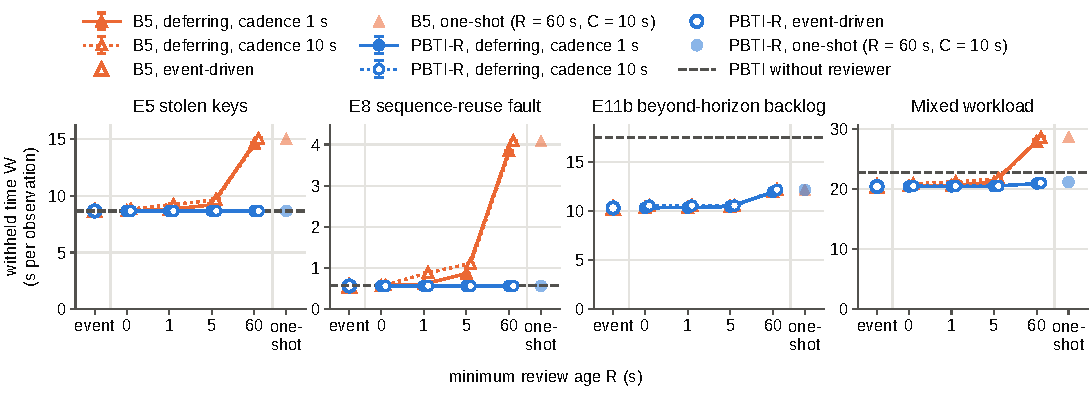
\includegraphics[width=\linewidth]{figures/fig_review_delay.pdf}
\end{adjustwidth}
\caption{Withheld time $W$ versus minimum review age $R$ (review-schedule evaluation; means of 20 paired seeds with 95\% bootstrap intervals). Colour marks the pipeline (B5 orange, PBTI-R blue); solid and dotted lines: deferring rule at 1~s and 10~s cadence; open markers at left: event-driven review; faded markers at right: one-shot rule with $R=60$~s and $C=10$~s; dashed line: \sys\ without reviewer. In E11b and the mixed workload the reviewer also recovers beyond-horizon data, which \sys\ keeps quarantined. Values: Table~\Sref{tab:S-a1-tests}.\label{fig:delay}}
\end{figure}

\subsection{Equivocation with Suppressed Messages and Selective Holds}\label{sec:res-selective}

Rule L cannot contest a forged version whose genuine version and successor never arrive: in the sensitivity factorial, equivocation combined with suppressed runs left \sys\ with \VFactPBTIOneFG\ non-legitimate observations per run, whereas B5's reviewer did not release them uncorroborated (\VFactBFiveOneFG). On the registered joint grid (Table~\Sref{tab:S-a3}, Figure~\Sref{fig:S-a3}), \sys\ retained forged observations at \WAthreePosPoints\ of the \WAthreePoints\ points, all with both equivocation and suppressed messages, and at most \WAthreePmaxOone\ per run. PBTI-SH retained none at \WAthreeSHzeroPoints\ of these points, yet gate G3 \WAthreeGThree: its reduction of O1 or NLX was better beyond the margin at only \WAthreeBetterPoints\ points, so gate G4 \WAthreeGFour\ either (descriptive breakdown in Table~\Sref{tab:S-gates}).

In the eight factorial cells added by the amendment (Table~\Sref{tab:S-a3f}, Figure~\Sref{fig:S-factorial}), PBTI-SH retained no forged observation in the four cells in which equivocation and suppressed runs coincide, against \WAthreeFPFGOone\ per run for \sys, \WAthreeFBfiveFGOone\ for \Bhist\ and \WAthreeFBfiveEvFGOone\ for \Bev; its exposure fell from \WAthreeFPFGNLX\ to \WAthreeFSHFGNLX\ record-seconds per run, better beyond the margin than \sys\ in all four cells, so gate G3F \WAthreeFGThree\ (through NLX), and G4F, which also requires withholding no worse than \Bhist, \WAthreeFGFour. The price was paid in genuine data: PBTI-SH withheld \WAthreeFSHFGW\ instead of \WAthreeFPFGW\ seconds per observation and finally missed \WAthreeFSHFGOtwo\ instead of \WAthreeFPFGOtwo\ legitimate observations per run, because an observation of a suspect feed whose successor never arrives stays withheld. The 30~s timeout variant gave the benefit up, releasing the withheld forgeries after the timeout (\WAthreeFSHTFGOone\ per run, as \sys). In the scenario controls (Table~\Sref{tab:S-a3-scen}), PBTI-SH had the same means as \sys\ on every primary outcome in \WAthreeSSameN\ of the \WAthreeSN\ workloads; it did not contain full impersonation (E5: \WAthreeSEfiveSHOone\ forged observations per run, as \sys) but withheld legitimate observations of forked feeds and after the benign sequence-reuse fault.

\subsection{Attacker-Model Sensitivity}\label{sec:res-attacker}

The impersonation attacker of the registered mixed workload is not fully consistent: transport duplicates of the genuine messages it suppresses reach the verifier, and a retransmitted or reordered forgery can contradict the attacker's own chain, so every pipeline received contradictions that a consistent attacker need not expose. An exploratory paired campaign repeated the mixed workload of the review-schedule evaluation on seeds 21--40 with an impersonator of the same capability (victims, window, keys, payload change) that re-sends one cached forgery per identity, chains predecessor links by sequence number and drops transport duplicates in the impersonated range (Table~\Sref{tab:S-v9-e04}). It raised the forged observations retained at the end of the run from \YEfourRegPBTIOOne\ to \YEfourConPBTIOOne\ per run for \sys\ and from \YEfourRegBhistOOne\ to \YEfourConBhistOOne\ for \Bhist, and the exposure of \sys\ from \YEfourRegPBTINLX\ to \YEfourConPBTINLX\ record-seconds. The ordering of the strategies persisted, but its size changed: the difference \Bhist\ minus \sys\ was \YEfourConBhistvsPBTINLX\ record-seconds of exposure per run (95\% CI [\YEfourConBhistvsPBTINLXLo, \YEfourConBhistvsPBTINLXHi]; \YEfourConBhistvsPBTINLXPct\% of the exposure of \sys, against \YEfourRegBhistvsPBTINLXPct\% under the registered attacker) and \YEfourConBhistvsPBTIW~s of withholding per observation, whereas with matched event-driven review B5 minus PBTI-R was \YEfourConBevvsRevNLX\ record-seconds of exposure and \YEfourConBevvsRevW~s of withholding (classes under the registered margins, used descriptively: \YEfourConBevvsRevNLXClass\ for exposure and \YEfourConBevvsRevWClass\ for withholding). The corrected and the historical B5 retained equally many forgeries in every seed and differed in these cell means by at most \YEfourHistCorrMaxOTwo\ lost observations, \YEfourHistCorrMaxNLX\ record-seconds of exposure and \YEfourHistCorrMaxW~s of withholding per run. Six deterministic control traces on the real verifiers (Table~\Sref{tab:S-v9-controls}) isolate the failure modes: every pipeline contests a forged version once a contradicting statement is admitted, and keeps it authoritative to the end when the successors are suppressed, when the attacker continues the feed consistently, when it writes identities that the device does not use, or when it opens a new epoch, after which the device's own statements are quarantined as stale until a reviewer, where present, releases them. Containment of either granularity therefore depends on contradicting evidence reaching the verifier, and the attack generator is a material source of uncertainty for retention and exposure magnitudes, which these runs do not settle for other workloads.

\subsection{Reviewed Release under Revoked Credentials}\label{sec:res-release}

The lifecycle analysis (Table~\Sref{tab:S-a5}) applies each release-evidence policy to the same hand-specified timelines on the real verifier, with keys compromised at $t_c$; \sys\ and B5 gave \WAfivePBTIBfiveSame\ results. The discretionary condition released a legitimate buffered record but also a backdated forgery produced with the compromised keys after $t_c$: a corroborating predecessor link satisfies the automated reviewer and a self-asserted time stamp the waiver, so the forgery became authoritative and, committed after the revocation had been processed, escaped taint. The witness policy refused the forgeries and released the legitimate record only when the witness had stamped its exact digest before the earliest plausible compromise time, accounting for the assumed witness-clock uncertainty; a witness outage withheld the record. Of the tested widths of the uncertainty interval around $t_c$, the record was recovered at \YEtenRecovered~s and withheld at \YEtenWithheld~s; these cases describe the specified record and witness timing and do not establish a general threshold. Under every policy and for every pipeline, a forgery contradicted by an admitted successor was rejected and a revoked reviewer could not decide; a decision bound to a superseded evidence snapshot was refused (at \YEnineRefusedAt~s, after new evidence had been admitted) and the case returned to quarantine, and the observation was recovered only through a later authorized decision on the current snapshot (at \YEnineFreshAt~s). The witness's key and clock are trusted by assumption, and the matrix is deterministic, not a campaign evaluation.

\subsection{Sensitivity Analyses, Replay, Audit and Ablation}\label{sec:res-sensitivity}

In the stressor sweep (Figure~\Sref{fig:S-sweep}), loss, duplicates, reordering, long delay and outages of up to 24~s changed neither outcome for any pipeline; B4 retained non-legitimate observations under equivocation (\VSwequivocationBFourOneTwenty\ per run at 20\%) and, lacking taint, after late compromise discovery, whereas \sys\ and B5 retained none and lost more legitimate observations instead, and B5 differed significantly from \sys\ in no sweep cell (exploratory), at the price of holds. In the replay of public test-bed telemetry (SKAB~\cite{katser2020skab}; Table~\Sref{tab:S-skab}), every replayed observation became authoritative in every pipeline in the unstressed controls, so process anomalies did not affect admission; with labelled stressors \sys\ and B5 retained \VRpOnePBTInonlegitauth\ and \VRpOneBFivenonlegitauth\ non-legitimate observations per run at native speed, against \VRpOneBFournonlegitauth\ for B4; in attributed re-runs, \VRpResPBTIgw\ of the \VRpResPBTItotal\ observations retained by \sys\ were forged by a compromised, never-revoked gateway for its legacy device, and \VRpResBFourimp\ of B4's \VRpResBFourtotal\ were impersonation that B4 cannot taint. The replay tests real sensor dynamics and timing, not attacks observed in a plant. The audit detected all seven insider tampering classes, including a rewrite re-signed with the evidence key, caught through the witness copies and decision replay (Table~\Sref{tab:S-audit}), and removing any one of the origin signature, the predecessor link, conflict detection, the horizon and epoch checks or revocation and taint significantly re-admitted non-legitimate observations on the mixed workload (\RAblnoprevlinknonlegitauth\ to \RAblnorevocationnonlegitauth\ per run versus \RAblfullnonlegitauth; Table~\Sref{tab:S-ablation}).

\subsection{Performance, Message Size and Resource Use}\label{sec:res-perf}

With SQLite group commit every 200 messages (write-ahead logging, \texttt{synchronous=\allowbreak{}NORMAL}), the in-process verifier sustained \RTpPBTI\ messages/s for \sys\ versus \RTpBOne, \RTpBTwo\ and \RTpBThree\ for B1--B3 on a two-vCPU host (\RTpRatioBTwo$\times$ B2); canonicalization, key lookup, hashing and the two Ed25519 verifications accounted for \XStageCryptoShare\% of the per-message cost (Figure~\Sref{fig:S-perf}c). Raising the commit batch from 1 to 128 raised single-process throughput only \VBtPBTIgainbatch-fold, consistent with signature verification dominating, and two or four verification workers raised it \VBtPBTIgainworkers- and \VBtPBTIgainworkersfour-fold at batch 128 with both vCPUs busy (Figure~\Sref{fig:S-perf}a,b; Table~\Sref{tab:S-batching}), with \VBatchSemanticsIdentical\ disposition sequences. A \sys\ message carried \RWirePBTI\ bytes on average against \RWireBTwo\ for B2 (\RWireRatioBTwo$\times$), of which the two signatures accounted for \XMbSigShare\% and the relay statement for \XMbRelShare\% (Table~\Sref{tab:S-bytes}); a binary encoding (CBOR, estimated, not implemented) would keep the ratio at \XMbBinTxtRatio--\XMbBinIntRatio$\times$. Persisted bytes per message were \RDbRatioBTwo$\times$ those of B2, resident memory grew by about 2.2~kB per message (B2: 0.7~kB) because verifier state is not pruned, and edge signing cost \REdgePBTI~$\mu$s of server CPU per message.

In the MQTT/TLS runs, with publisher, broker and verifier sharing two vCPUs (Figure~\Sref{fig:S-perf}d; Table~\Sref{tab:S-e2e2}), the median publication-to-commit latency at 1000 messages/s was \VEePBTIrOneZeroZeroZeropfifty~ms for \sys\ and \VEeBTworOneZeroZeroZeropfifty~ms for B2 (p99 \VEePBTIrOneZeroZeroZeropninetynine\ versus \VEeBTworOneZeroZeroZeropninetynine~ms); offered 1250 and 1500 messages/s, the \sys\ verifier committed \VEePBTIrOneTwoFiveZerotp\ and \VEePBTIrOneFiveZeroZerotp~messages/s, whereas B2 kept up, and the SKAB replay stayed far below saturation (Table~\Sref{tab:S-e2e-skab}). Because the co-located roles used about 1.7 of the two vCPUs at 1000 messages/s, these runs locate the saturation of the shared host, not the capacity of a dedicated verifier, and with 10~s measurement windows starting from an empty store they do not establish a sustainable rate.
